\chapter{Project Design}
\label{ch:design}

This chapter specifies the requirements, shows the system context and data flow, presents the user interface, and then details the research methodology: data and point-in-time alignment, the baseline memories, our self-correcting memory with its seven components, the decision policies, the extension models, the safe-autonomy design of the application and the evaluation protocol. It ends with the alternatives we considered, the project plan and the task allocation.

\section{Requirement Analysis}
\subsection{Functional and Nonfunctional Requirements}
\paragraph{Functional requirements.}
\begin{enumerate}
  \item[FR1] Download news, SEC filings and daily prices for a configurable ticker universe and align every item to the first trading session at which it was public.
  \item[FR2] Annotate every text with polarity and an embedding, identically for all memory systems.
  \item[FR3] Replay Plain RAG, FinMem and the proposed memory day by day and log retrieved evidence, signals and memory operations.
  \item[FR4] Evaluate rule, ML and LLM policies under rolling and fixed protocols with costs, statistics and ablations; export tables and figures.
  \item[FR5] For a selected ticker, show the retrieved memories with layer, age, polarity, credibility and corroboration, the episodic and peer evidence, and the signals of all three memories.
  \item[FR6] Produce a recommendation from the memory signal and a price model, query a chosen LLM backbone with the same prompt as the study, and highlight the memories it cites.
  \item[FR7] Execute approved decisions on an Alpaca paper account (or a local simulated account) under position and loss limits.
  \item[FR8] Refresh data incrementally and rebuild the memory from the application.
  \item[FR9] Present study results interactively (equity curves, tables, tests, heatmaps, figures).
  \item[FR10] Let the user set a trading budget and hard limits (cash reserve, per-stock cap, single-order cap, daily-loss and drawdown limits, trades per day, allowed stocks) that every automated order must respect.
  \item[FR11] Run the agent autonomously on a schedule with a selectable permission mode (suggest only, approval required, guarded automatic, fully automatic) and decision mode (rules, LLM, both must agree), an approval queue and an emergency stop.
  \item[FR12] Suggest how to split the budget across stocks (risk parity, minimum variance, equal weight, signal-tilted) with a walk-forward comparison, and turn a plan into orders that wait for approval.
  \item[FR13] Provide analytics for the selected stock: chart-pattern analogues and their back-test, return distribution and risk, correlation, Monte Carlo equity distribution, and an algorithm board showing what every evaluated model says today with its out-of-sample track record and decision log, including a reinforcement-learning agent.
  \item[FR14] Let a non-technical user connect broker and LLM accounts by pasting API keys, which are verified with the provider before they are stored.
  \item[FR15] Offer the whole interface in English and Bangla, in light and dark themes, on desktop and mobile.
\end{enumerate}
\paragraph{Nonfunctional requirements.}
\begin{itemize}
  \item \textbf{No look-ahead}: no component may use information published after the decision time (enforced by tests).
  \item \textbf{Reproducibility}: every reported number is generated by code from versioned data; LLM responses are cached by prompt hash.
  \item \textbf{Cost}: runs on a laptop CPU (8 cores, 8\,GB RAM) using free data and inference tiers.
  \item \textbf{Safety}: paper trading by default; live trading requires two explicit opt-ins; every agent order passes one server-side guardrail; risk-reducing exits are never blocked by trade-count limits; an emergency stop cancels pending orders.
  \item \textbf{Security}: API keys stay on the user's machine in an owner-only file, are never returned to the browser in full, and can only be read or changed from the application's own page on the same machine.
  \item \textbf{Usability and accessibility}: plain-language explanations next to every metric, bilingual interface, light/dark themes, responsive layout, colour never the only carrier of meaning.
  \item \textbf{Transparency}: every decision exposes its evidence; limitations of the study are shown in the application.
  \item \textbf{Maintainability}: modular package with automated tests (\testcount{} tests).
\end{itemize}

\subsection{Context Diagram}
\begin{figure}[H]
\centering
\begin{tikzpicture}[node distance=1.6cm and 2.4cm, every node/.style={font=\small},
  sys/.style={circle, draw, thick, fill=blue!8, minimum size=3.2cm, align=center},
  ext/.style={rectangle, draw, rounded corners, fill=gray!10, minimum width=3.0cm, minimum height=0.9cm, align=center},
  arr/.style={-{Latex[length=2mm]}, thick}]
\node[sys] (s) {Agentic Trade\\ memory agent\\ \& application};
\node[ext, above left=of s] (user) {Trader / researcher};
\node[ext, above right=2.0cm and 3.2cm of s] (alpaca) {Alpaca\\ (news, bars,\\ paper broker)};
\node[ext, below right=2.0cm and 3.2cm of s] (sec) {SEC EDGAR\\ (XBRL filings)};
\node[ext, below left=of s] (llm) {LLM providers\\ (Groq, OpenRouter)};
\draw[arr] (user) to[bend left=10] node[above, sloped]{ticker, approval} (s);
\draw[arr] (s) to[bend left=10] node[below, sloped]{evidence, advice} (user);
\draw[arr] (alpaca) to[bend right=10] node[above, sloped]{news, prices, fills} (s);
\draw[arr] (s) to[bend right=10] node[below, sloped]{paper orders} (alpaca);
\draw[arr] (sec) -- node[below, sloped]{10-Q / 10-K facts} (s);
\draw[arr] (s) to[bend left=10] node[above, sloped]{prompt} (llm);
\draw[arr] (llm) to[bend left=10] node[below, sloped]{decision JSON} (s);
\end{tikzpicture}
\caption{Context diagram.}
\label{fig:context}
\end{figure}

\subsection{Data Flow Diagram Level 1}
\begin{figure}[H]
\centering
\begin{tikzpicture}[every node/.style={font=\footnotesize},
  proc/.style={circle, draw, thick, fill=blue!8, minimum size=1.9cm, align=center, inner sep=1pt},
  store/.style={draw, thick, fill=white, minimum width=2.4cm, minimum height=0.6cm, align=center, path picture={\draw (path picture bounding box.north west) -- (path picture bounding box.south west);}},
  ext/.style={rectangle, draw, fill=gray!10, minimum width=2.2cm, minimum height=0.7cm, align=center},
  arr/.style={-{Latex[length=1.8mm]}, thick}]
% row 1: ingest and annotate
\node[ext]   (src) at (0,0)      {Alpaca / SEC};
\node[proc]  (p1)  at (3.1,0)    {1.0\\ Ingest \&\\ align (PIT)};
\node[store] (d1)  at (6.25,0)   {D1 raw data};
\node[proc]  (p2)  at (9.4,0)    {2.0\\ Annotate\\ (FinBERT,\\ MiniLM)};
% row 2: memory replay and evaluation
\node[store] (d2)  at (9.4,-2.7) {D2 annotated};
\node[proc]  (p3)  at (6.25,-2.7){3.0\\ Memory\\ replay};
\node[store] (d3)  at (3.1,-2.7) {D3 signals \&\\ evidence};
\node[proc]  (p5)  at (0,-2.7)   {5.0\\ Evaluate \&\\ report};
% row 3: decision
\node[proc]  (p4)  at (3.1,-5.4) {4.0\\ Decide\\ (rule, ML,\\ LLM)};
\node[ext]   (llm) at (6.25,-5.4){LLM API};
% row 4: user and execution
\node[ext]   (user) at (3.1,-8.1){User};
\node[proc]  (p6)  at (6.25,-8.1){6.0\\ Execute\\ (paper)};
\draw[arr] (src) -- (p1);
\draw[arr] (p1) -- (d1);
\draw[arr] (d1) -- (p2);
\draw[arr] (p2) -- (d2);
\draw[arr] (d2) -- (p3);
\draw[arr] (p3) -- (d3);
\draw[arr] (d3) -- (p5);
\draw[arr] (d3) -- (p4);
\draw[arr] (llm) -- node[above]{decision} (p4);
\draw[arr] (p4) -- node[above right]{order} (p6);
\draw[arr] (user) -- node[left]{approve} (p4);
\draw[arr] (p6) -- node[below]{fills} (user);
\draw[arr] (p5) |- node[pos=0.3, right]{tables, figures} (user);
\end{tikzpicture}
\caption{Level-1 data flow diagram.}
\label{fig:dfd}
\end{figure}

\subsection{UI Design}
The application is a single-page web interface served by a dependency-free Python HTTP server. It was designed for users without a finance or computing background. A sidebar groups the pages into \emph{Main} (Home, Trade, Portfolio, AI Autopilot, Insights), \emph{Research} (Stock scanner, AI memory, Research lab) and Settings. One stock picker in the top bar drives every page, so the user chooses a stock once and every view follows it. Every metric has a plain-language explanation, the interface can be switched between English and Bangla and between light and dark themes, and on a phone the sidebar becomes a bottom navigation bar (Appendix~\ref{app:guide}). Colours come from one set of design tokens per theme, so charts and tables follow the theme, and colour is never the only carrier of meaning: every green or red value also carries a sign, a label or an icon. The main pages are described below; the analytics pages are shown with the results they implement in Chapter~\ref{ch:impl}. All screenshots in this report use the light theme, whose text colours were chosen to stay legible in print.

\paragraph{Home.} The Home page (Figure~\ref{fig:ui-home}) answers three questions a user has when opening the application: how much money is there, what is the AI doing, and is anything at risk. The top card shows the total account value with cash, invested amount, open profit or loss and the number of stocks held, and a badge states whether the account is the Alpaca paper account or the local simulator. Next to it, the autopilot card shows whether the agent is running, its permission level, how it decides and how many trades are waiting for approval. The ``AI view'' card turns the research agent's output for the selected stock into one word (Buy, Sell or Hold), a confidence value and one plain sentence, together with the last close, the 20-day move, the price model's chance of a rise and the number of articles read that day; it also reminds the user that the study found these signals only weakly predictive. The budget card shows, as progress bars, how much of the budget is in use, today's loss against the daily limit and the drop from the account's peak, and the activity list shows the latest orders and decisions.
\begin{figure}[!htbp]
\centering
\appshot{app_home_paper.png}
\caption{Home: account value, autopilot status, the agent's view of the selected stock in plain words, budget and safety meters and recent activity.}
\label{fig:ui-home}
\end{figure}

\paragraph{Trade.} The Trade page (Figure~\ref{fig:ui-terminal}) is where a user looks at one stock and places an order by hand. The chart shows the real daily candles of the selected stock with optional 20- and 50-day averages, volatility bands, RSI and MACD. Four classic indicators (RSI, MACD, trend and position in the recent range) are explained in words and combined into one score on a bearish--bullish scale, so that a beginner does not have to read the indicators separately. The ``Ask the AI agent'' button requests a decision from the research agent and, if the user agrees, executes it within the budget limits. The position card shows shares, average price and profit or loss with one-click ``sell all'' and ``sell half'' buttons, and the order ticket accepts an amount in dollars or shares, suggests 5, 10 or 25\% of the cash and shows the estimated number of shares before the order is sent.
\begin{figure}[!htbp]
\centering
\appshot{app_trade_paper.png}
\caption{Trade: real daily candles with moving averages, four chart signals combined into one score, the AI decision button, the current position and an order ticket in dollars or shares.}
\label{fig:ui-terminal}
\end{figure}

\paragraph{AI Autopilot.} The AI Autopilot page (Figure~\ref{fig:ui-autopilot}) controls the agent's autonomy (Section~\ref{sec:autopilot-design}). The top bar states in one sentence whether the autopilot is running and offers three buttons: start, run one check now, and an emergency stop that is always visible in red. Below it, the live safety limits show how close the account is to each hard limit and what happens when it is reached (for example, new buys stop for the day, while selling to reduce risk is always allowed). The approval queue lists the trades that wait for the user's decision; each one is re-checked against the limits when it is approved. The four permission levels are presented as cards ordered from safest to most autonomous, each with a one-line explanation, and the decision mode (rules only, the language model, or both must agree) and the schedule (how often to check, how many stocks per check, the buy size and whether to trade only while the U.S.\ market is open) are set below. The activity log at the bottom records every decision and what happened to it.
\begin{figure}[!htbp]
\centering
\appshot{app_autopilot_paper_1.png}
\caption{AI Autopilot: state and controls, live safety limits, approval queue, permission modes, decision modes and schedule.}
\label{fig:ui-autopilot}
\end{figure}
\begin{figure}[!htbp]
\ContinuedFloat
\centering
\appshot{app_autopilot_paper_2.png}
\caption[]{(continued)}
\end{figure}

\paragraph{Budget and limits.} The budget form in Settings (Figure~\ref{fig:ui-budget}) is the single place where the user sets the hard limits that every automated order must respect: the total budget the AI may manage, the share always kept as cash, the maximum in one stock and in one order, the daily loss and drawdown limits, the number of trades per day and the stocks the AI may buy. Each field has a one-line explanation, and a sentence under the form restates all limits in dollars (for example, ``The AI may invest up to \$8{,}000 of your \$10{,}000 \ldots''), so that the user can check the effect of a percentage before saving it. The other Settings tabs hold the broker and LLM connections, whose keys are verified before they are stored, and the language and theme preferences.
\begin{figure}[!htbp]
\centering
\appshot{app_budget_paper.png}
\caption{Settings, Budget \& limits: the hard limits every automated order must respect, with a plain-language summary.}
\label{fig:ui-budget}
\end{figure}

\paragraph{AI memory.} The AI memory page (Figure~\ref{fig:ui-agent}) opens the research agent for inspection and is the application's link to the study. The summary cards show the memory signal and its decision threshold, the recommendation and its confidence, the price model's chance of a rise, the outcome of similar past situations (N7) and the signal from related companies (N6). The left column lists what the agent remembers, grouped by memory layer, and every memory shows its date, age, tone, learned credibility (N1), headline category, author and identifier, so that a user can verify the evidence behind a decision. The right column explains the recommendation, compares the three memory designs of the study (Plain RAG, FinMem and ours) on the same day's data, and plots the price together with the memory signal and its threshold over the last 90 days. From this page the user can ask a chosen LLM backbone for a decision with the same prompt as the study; the memories it cites are highlighted.
\begin{figure}[!htbp]
\centering
\appshot{app_memory_paper.png}
\caption{AI memory: the memories retrieved by our agent per layer with tone, credibility and corroboration (left); recommendation, the three memory designs compared and the signal history (right).}
\label{fig:ui-agent}
\end{figure}

\paragraph{Stock scanner.} The scanner (Figure~\ref{fig:ui-scanner}) shows all ten stocks in one table: price, one-day and 20-day change, the memory signal as a bar, the action of our memory (including when it abstains), FinMem's action, the price model's probability of a rise, the combined recommendation and its confidence. Because the recommendation only says Buy or Sell when the memory agent and the price model agree, most rows show Hold, which reflects the weak signals found in the study. A row opens the AI memory page for that stock, and one button sends all current recommendations to the approval queue.
\begin{figure}[!htbp]
\centering
\appshot{app_scanner_paper.png}
\caption{Stock scanner: memory signal, FinMem action, price-model probability and consensus for all ten stocks.}
\label{fig:ui-scanner}
\end{figure}

\paragraph{Research lab.} The Research lab (Figure~\ref{fig:ui-research}) presents the results of this report interactively. The user chooses the evaluation protocol (rolling walk-forward or fixed split) and the stock set (all ten or FinMem's five); headline cards then show our Sharpe ratio, return and worst fall against FinMem, the Sharpe gain and its significance. The equity chart shows the growth of \$1 for every strategy, with a legend that switches strategies on and off, and the tables below list all strategies and the significance tests of ours against each baseline, followed by per-stock results and the model comparison of Section~\ref{sec:ext-results}. The numbers are read from the same result files as the tables of Chapter~\ref{ch:impl}.
\begin{figure}[!htbp]
\centering
\appshot{app_research_paper_1.png}
\caption{Research lab: headline statistics, interactive equity curves, all-strategy table and significance tests of the study.}
\label{fig:ui-research}
\end{figure}
\begin{figure}[!htbp]
\ContinuedFloat
\centering
\appshot{app_research_paper_2.png}
\caption[]{(continued)}
\end{figure}

\paragraph{Insights.} The Insights page groups the analytics into six tabs: budget split (Figure~\ref{fig:ui-split}), pattern finder (Figure~\ref{fig:ui-pattern}), what-if, risk, correlation, and the algorithm board with the reinforcement-learning agent (Figures~\ref{fig:ui-algo}--\ref{fig:ui-rl}). They are shown in Chapter~\ref{ch:impl} together with the experiments they are based on.

\section{Detailed Methodology and Design}

\subsection{System architecture}
\begin{figure}[H]
\centering
\begin{tikzpicture}[every node/.style={font=\footnotesize},
  box/.style={rectangle, draw, rounded corners, thick, align=center, minimum height=0.85cm},
  nov/.style={box, fill=blue!10, minimum width=2.7cm},
  arr/.style={-{Latex[length=1.8mm]}, thick}]
\node[box, fill=gray!10, text width=12.4cm, align=center] (data) at (0,0) {News (Alpaca/Benzinga) \quad 10-Q/10-K (SEC XBRL) \quad Daily prices $\rightarrow$ point-in-time alignment, FinBERT, MiniLM};
\node[box, fill=orange!10, text width=12.4cm, align=center] (fm) at (0,-1.4) {FinMem core: shallow/intermediate/deep layers, $Q=14/90/365$, importance $v\alpha^\delta$, purge, access counter \& promotion, top-$K$ per layer};
\node[nov] (n1) at (-4.8,-2.9) {N1 credibility};
\node[nov] (n2) at (-1.6,-2.9) {N2 dedup};
\node[nov] (n3) at (1.6,-2.9) {N3 contradiction};
\node[nov] (n4) at (4.8,-2.9) {N4 situational query};
\node[nov] (n5) at (-4.8,-4.0) {N5 importance};
\node[nov] (n6) at (-1.6,-4.0) {N6 peer graph};
\node[nov] (n7) at (1.6,-4.0) {N7 episodic recall};
\node[box, fill=green!8, minimum width=2.7cm] (agg) at (4.8,-4.0) {weighted aggregation};
\node[draw, dashed, rounded corners, fit=(n1)(n4)(n5)(agg), inner sep=5pt, label={[font=\footnotesize]above right:{Ours}}] (ours) {};
\node[box, fill=gray!10, text width=12.4cm, align=center] (pol) at (0,-5.7) {Decision: threshold rule \quad | \quad LightGBM / LogReg \quad | \quad LLM backbones (FinMem-style prompt) $\rightarrow$ Buy / Sell / Hold};
\node[box, text width=12.4cm, align=center] (out) at (0,-7.0) {Evaluation (rolling \& fixed, costs, tests) \qquad Application (inspect, consensus, paper execution)};
\draw[arr] (data) -- (fm);
\draw[arr] (fm) -- (ours.north);
\draw[arr] (ours.south) -- (pol);
\draw[arr] (pol) -- (out);
\end{tikzpicture}
\caption{Architecture of the study and of the proposed memory (``Ours'' = FinMem core plus N1--N7).}
\label{fig:arch}
\end{figure}

\subsection{Data and point-in-time alignment}
The universe is FinMem's five stocks (TSLA, NFLX, AMZN, MSFT, COIN) plus NVDA, AAPL, GOOGL, META and AMD. Table~\ref{tab:data} and Figure~\ref{fig:data} summarise the data.
\begin{itemize}
  \item \textbf{News}: all articles tagged with any universe ticker by the Alpaca News API (Benzinga), 1 September 2025 -- 27 October 2026: headline, summary, author, symbol list and timestamp.
  \item \textbf{Filings}: every 10-Q and 10-K filed since July 2024, from SEC EDGAR XBRL company facts. Since we do not use an LLM to summarise filings, each filing is rendered as a short factual text (revenue, net income, diluted EPS with year-over-year change, operating margin) and its polarity is $\tanh(3\cdot\text{mean YoY growth})$.
  \item \textbf{Prices}: split- and dividend-adjusted consolidated daily bars for the ten stocks, SPY and QQQ.
\end{itemize}
An item becomes visible at the close of the first trading day whose 16:00 New York close is at or after its timestamp; after-hours news therefore belongs to the next session, and filings become visible after the close of their filing day. Decisions are taken at the close of day $t$ and earn the return from close $t$ to close $t+1$; outcomes of day-$t$ decisions are resolved only at close $t+1$, before the day-$(t+1)$ decision.

\begin{table}[ht]
\centering
\caption{Dataset composition: articles tagged with each ticker (an article can mention several), and SEC filings since July 2024.}
\label{tab:data}
\begin{tabular}{lrrr}
\hline
Ticker & News articles & 10-Q & 10-K \\
\hline
TSLA & 4,541 & 8 & 2 \\
NFLX & 1,161 & 8 & 2 \\
AMZN & 4,381 & 7 & 2 \\
MSFT & 4,263 & 6 & 3 \\
COIN & 1,211 & 7 & 2 \\
NVDA & 6,819 & 7 & 2 \\
AAPL & 3,486 & 7 & 2 \\
GOOGL & 4,568 & 7 & 2 \\
META & 3,815 & 8 & 2 \\
AMD & 1,839 & 7 & 2 \\
\hline
Unique total & 23,247 & 72 & 21 \\
\hline
\end{tabular}
\end{table}


\begin{figure}[H]
\centering
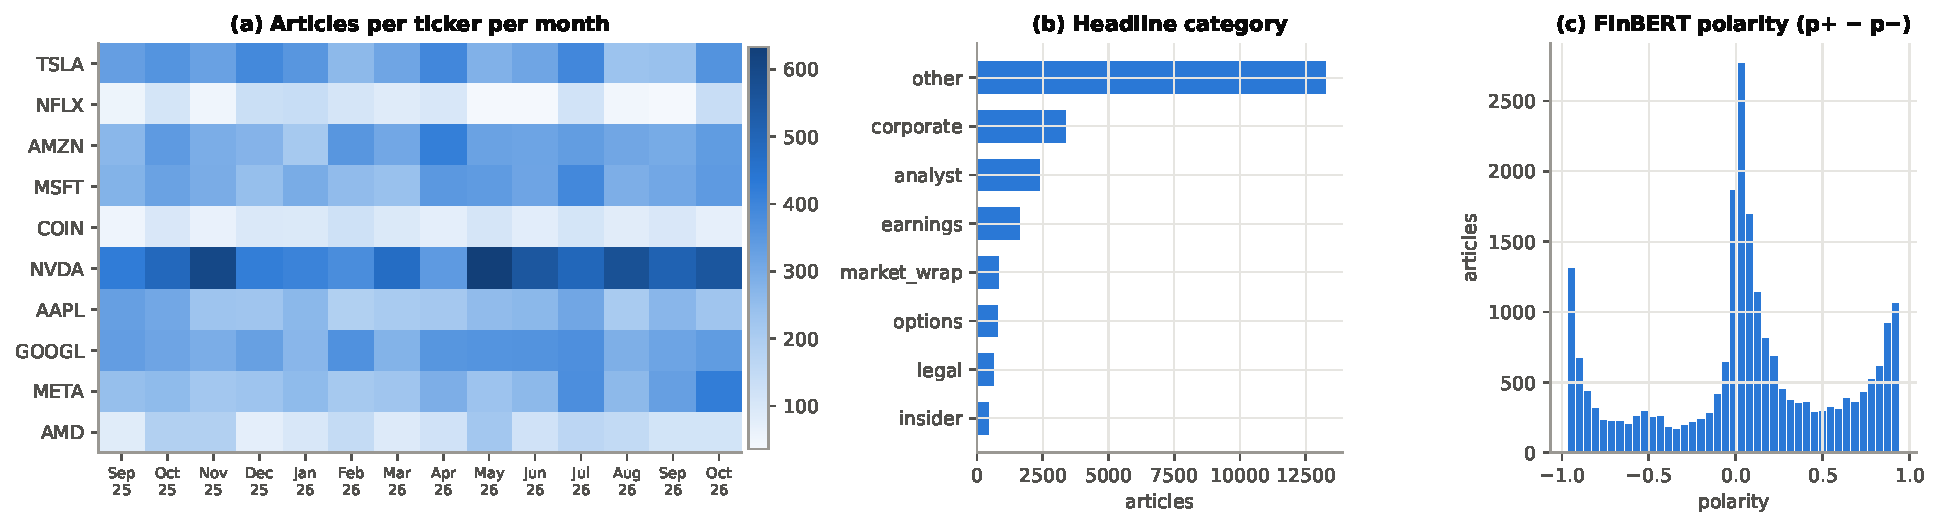
\includegraphics[width=\textwidth]{fig01_data_overview.pdf}
\caption{Dataset overview: (a) articles per ticker per month, (b) headline categories used by credibility learning, (c) distribution of FinBERT polarity.}
\label{fig:data}
\end{figure}

\subsection{Shared annotation}
Each headline receives a FinBERT polarity $s\in[-1,1]$ and each headline plus summary a unit-length MiniLM embedding $\mathbf{e}$. Headlines are also assigned a coarse category (analyst, earnings, options, insider, legal, market wrap, corporate, other) by keyword rules; this category is used only by N1. Every system receives exactly the same annotations.

\subsection{Baseline memories}
\label{sec:finmem-impl}
Both baselines use exactly the same data and annotations as our memory, so that every difference comes from the memory design.

\paragraph{Faithful FinMem.} We implement FinMem's scoring as described in Section~\ref{sec:finmem-bg}: recency $e^{-\delta/Q_l}$, relevancy $\mathbf{e}_E\cdot\mathbf{q}$ where $\mathbf{q}$ embeds the trading inquiry (``Can you make an investment decision on Tesla (TSLA) stock? \dots''), importance $\min(1,(v+b)\alpha_l^{\delta}/100)$ with $v$ drawn from FinMem's layer probabilities ($\{0.8,0.15,0.05\}$, $\{0.05,0.8,0.15\}$, $\{0.05,0.15,0.8\}$ over $\{40,60,80\}$) and $b$ the access-counter bonus. News enters the shallow layer, 10-Qs the intermediate and 10-Ks the deep layer. Shallow memories are purged when recency $<0.05$ or importance $<5$. After each outcome is known, the top-3 retrieved memories whose polarity sign matched the realised return receive $b \mathrel{+}= 5$; a memory whose $v+b$ reaches 60 (80) moves to the intermediate (deep) layer and its recency is reset. The top $K=5$ memories of each layer are retrieved. Deviations from the original are deliberate and apply equally to all systems: open encoders instead of GPT summaries and \texttt{ada-002} embeddings, and no purging in the intermediate and deep layers, which hold the filings (FinMem keeps a report for its reporting cycle) and promoted news.

\paragraph{Plain RAG baseline.} A single pool with recency $e^{-\delta/14}$ plus relevancy and the top 5 items overall, in the spirit of Generative Agents without importance or layers.

\subsection{Proposed self-correcting memory (N1--N7)}
Our memory (called ``Ours'' in tables and figures) keeps the layered core described above and adds seven components, each of which can be switched off for ablation. They follow the \emph{remember--verify--act} idea of Chapter~\ref{ch:intro} (Table~\ref{tab:rva}): N2, N4, N5 and N6 decide what is stored and retrieved, N1, N3 and N7 check whether a memory should be trusted or acted on, and the decision policies and guardrails turn the verified context into an action.
\begin{table}[H]
\centering
\caption{The seven components of our memory grouped by role.}
\label{tab:rva}
\small
\begin{tabular}{p{0.13\textwidth}p{0.34\textwidth}p{0.45\textwidth}}
\hline
Role & Component & What it fixes \\
\hline
Remember & N2 near-duplicate consolidation & the same story stored many times \\
 & N4 situational query & retrieval ignores what is happening today \\
 & N5 data-driven importance & importance drawn at random \\
 & N6 point-in-time peer graph & news about related companies ignored \\
\hline
Verify & N1 hierarchical source credibility & every source trusted equally \\
 & N3 contradiction retirement & contradicted facts kept until they decay \\
 & N7 outcome-aware episodic recall & no learning from the agent's own outcomes \\
\hline
Act & decision policies, guardrails & rule, ML and LLM decisions; budget limits and approvals in the application \\
\hline
\end{tabular}
\end{table}

\paragraph{N1 -- Hierarchical online source credibility.} For every visible article with $|s|\ge 0.2$, once its next-day outcome is known we record a hit if $\operatorname{sign}(s)=\operatorname{sign}(r_{t+1}-r^{\text{SPY}}_{t+1})$ (market-adjusted). Credibility is a Beta--Bernoulli posterior shrunk from author to category to global:
\begin{equation}
c_g=\frac{h_g+m\cdot 0.5}{n_g+m},\qquad c_k=\frac{h_k+m\,c_g}{n_k+m},\qquad c_a=\frac{h_a+m\,c_k}{n_a+m},
\end{equation}
with prior strength $m=8$, where $h$ and $n$ are hits and observations for the global pool $g$, the headline category $k$ and the author $a$. Credible memories gain $2(c-0.5)$ in retrieval score and enter the signal with weight $w=\operatorname{clip}(2(c-0.5),0,1)+0.05$. Updates use only resolved outcomes, so the estimate is point-in-time.

\paragraph{N2 -- Near-duplicate consolidation.} An incoming item whose embedding has cosine similarity $\ge 0.88$ with an active memory of the same layer and the same polarity sign does not create a new memory; instead the stored memory's corroboration count $n_c$ increases and its timestamp is refreshed. Corroboration adds $10\ln n_c$ importance points and multiplies the evidence weight by $1+\ln n_c$.

\paragraph{N3 -- Semantic contradiction retirement.} If a new item with $|s|\ge 0.3$ has similarity $\ge 0.72$ with an older active memory of the same layer whose polarity is opposite and $|s|\ge 0.3$, the older memory is retired.

\paragraph{N4 -- Situational query.} The query is $\mathbf{q}=\operatorname{normalize}(\mathbf{q}_{\text{task}}+\bar{\mathbf{e}}_{\text{today}})$, where $\bar{\mathbf{e}}_{\text{today}}$ is the mean embedding of the ticker's articles of the day, so that retrieval looks for memories related to what is happening now.

\paragraph{N5 -- Data-driven importance.} Instead of a random draw, $v = 40 + 40\cdot\operatorname{clip}\!\big(0.5|s|+0.5\tanh(a-1),0,1\big) + 20\,l$, where $a=(n_{\text{today}}+1)/(\bar n_{20}+1)$ is the news-attention surprise relative to the previous 20 sessions and $l\in\{0,1,2\}$ the layer index.

\paragraph{N6 -- Point-in-time peer graph.} Articles naming two to six symbols form a co-mention graph over a rolling 120-day window (only past days). The three most co-mentioned universe peers receive weights $w_p$ proportional to their counts; up to three same-day articles about each peer that do not mention the focal ticker, chosen by similarity to the query, contribute with weight $0.5\,w_p\,w(c)$.

\paragraph{N7 -- Outcome-aware episodic memory.} Every decision stores an episode: the context vector (weighted mean embedding of the retrieved memories), the signal $S$ and the realised market-adjusted return $\tilde r$. At decision time the ten most similar past contexts with similarity $>0.3$ are recalled; if at least five exist, the edge is
\begin{equation}
\epsilon=\frac{\sum_j \text{sim}_j\,\operatorname{sign}(S_j)\,\tilde r_j}{\sum_j \text{sim}_j},
\end{equation}
and the agent abstains (keeps its position) when $\epsilon<0$, i.e.\ when acting on the news signal in similar situations lost money.

\paragraph{Evidence aggregation.} For retrieved memories $i$ (and peer items) with polarity $s_i$ and weight $w_i$ ($w_i=1$ for the baselines), the memory signal is
\begin{equation}
S=\frac{\sum_i w_i s_i}{\sum_i |w_i|}\in[-1,1].
\end{equation}

\subsection{Decision policies}
\begin{itemize}
  \item \textbf{Threshold rule (all memories).} Buy if $S>\theta$, Sell if $S<-\theta$, otherwise Hold, with FinMem's semantics: Buy holds a long position, Sell a short position, Hold keeps the current position. $\theta\in\{0,0.05,0.1,0.15,0.2,0.3,0.4\}$ is chosen per system (Section~\ref{sec:protocols}).
  \item \textbf{Rule baselines.} Buy-and-hold; 1-day momentum; 20-day time-series momentum; 5-day mean reversion; 20-day moving-average crossover; and the sign of the day's average headline polarity (no memory).
  \item \textbf{Learned baselines.} Logistic regression and LightGBM~\cite{ke2017lightgbm} predicting the sign of the next-day return from nine price features (1/5/20-day returns, 20-day volatility, RSI, distance to the 20-day average, volume z-score, SPY 1/5-day returns), optionally with FinMem's or our memory features. Long when $P(\text{up})>0.5+\mu$, short when $<0.5-\mu$.
  \item \textbf{LLM backbones.} The retrieved memories (with credibility and corroboration tags and the peer and episodic summaries for ours), 3-day momentum, the current position and FinMem's self-adaptive character are rendered into a prompt; the model returns JSON with action, confidence, reasoning and cited memory IDs. We use three free models on Groq, \texttt{gpt-oss-120b}, \texttt{gpt-oss-20b} and \texttt{qwen3.8-27b}, with temperature 0 and no cross-model fallback. OpenRouter's free models were tried but dropped: on a free account all free models share a cap of 50 requests per day, and the one uncapped model we found was throttled upstream to about 30 requests per hour.
\end{itemize}

\subsection{Extension models}
\label{sec:ext-design}
To test whether the conclusions depend on the model family, we added five models that use the same (ticker, date) grid, the same test window, monthly walk-forward re-fitting, the same probability margin $\mu=0.02$ and the same 5\,bps costs as LightGBM. All settings were fixed before the first run.
\begin{itemize}
  \item \textbf{GRU (price).} For every (ticker, day), the nine price features of the last $L=20$ trading days are standardised with training-window statistics, clipped to $\pm5$ and fed to a one-layer GRU with 32 hidden units and a 4-dimensional ticker embedding; the last hidden state gives $P(\text{up})$ through a linear layer.
  \item \textbf{Transformer (price).} The same window is projected to $d=32$, a learned positional embedding and a ticker embedding are added, and two Transformer encoder layers (2 heads, feed-forward size 64, dropout 0.1) process it; the representation of the decision day predicts $P(\text{up})$ (Figure~\ref{fig:transformer-arch}).
  \item \textbf{Transformer (price+memory).} The same network with our memory features (signal, day sentiment, number of articles, conflict, redundancy, mean age, layer counts, peer signal, episodic edge, mean credibility) added to every day of the window.
  \item \textbf{Training.} Binary cross-entropy on the sign of the next-day return, AdamW~\cite{loshchilov2019adamw} (learning rate $10^{-3}$, weight decay $10^{-3}$), batch 64, gradient clipping 1.0, at most 40 epochs with early stopping (patience 6) on the last 15\% of the training rows in time order; three seeds are averaged, as for LightGBM. The model is refitted at the start of every test month on all labels that were resolved before the month began.
  \item \textbf{RL Q-learning.} A tabular agent (Section~\ref{sec:rl-bg}) with state $s=(\text{5-day move}\in\{\downarrow,\approx,\uparrow\}$ at $\pm2\%$, price above/below its 20-day average, RSI band $<35$/$35$--$65$/$>65$, current position$)$, i.e.\ 36 states, and actions Flat or Long. The reward is the next-day return of the chosen position minus 5\,bps per switch; $\alpha=0.1$, $\gamma=0.9$. It pre-trains for 30 passes on the history of all ten stocks before December 2025 with $\varepsilon$ decaying from 1 to 0.05, then trades the test window greedily. After each day's return becomes known it updates $Q$ from that day's experience of all ten stocks; because the market return does not depend on the agent, the rewards of both actions are known and both are learned from.
  \item \textbf{Pattern analogues (kNN).} For each stock and day, the 8 most similar past 20-day windows of the same stock (Pearson correlation of z-normalised log prices, non-overlapping, outcome fully observed) vote with similarity weights on the 10-day forward return; Buy if the expected move exceeds 1\% and $P(\text{up})\ge0.55$, Sell if it is below $-1\%$ and $P(\text{up})\le0.45$, otherwise Hold. These are the application's default settings, chosen before any test result.
  \item \textbf{Exploratory combinations} (defined \emph{after} the main results and reported separately): a \emph{risk overlay} that takes LightGBM's position but stays in cash whenever our memory abstains (N7), and a \emph{model vote} that takes the majority sign of LightGBM, the Transformer and our memory.
\end{itemize}

\begin{figure}[H]
\centering
\begin{tikzpicture}[every node/.style={font=\footnotesize},
  box/.style={rectangle, draw, rounded corners, thick, align=center, minimum height=0.8cm},
  arr/.style={-{Latex[length=1.8mm]}, thick}]
\node[box, fill=gray!10, minimum width=3.2cm] (in) at (0,0) {20 days $\times$ 9 price\\features (z-scored)};
\node[box, fill=blue!8, minimum width=3.0cm] (proj) at (4,0) {Linear $9\!\to\!32$\\+ position + ticker emb.};
\node[box, fill=violet!12, minimum width=3.0cm] (enc1) at (8,0) {Encoder layer 1\\2-head attention + FFN};
\node[box, fill=violet!12, minimum width=3.0cm] (enc2) at (8,-1.5) {Encoder layer 2\\2-head attention + FFN};
\node[box, fill=green!10, minimum width=3.0cm] (head) at (4,-1.5) {LayerNorm + Linear\\on decision day};
\node[box, fill=gray!10, minimum width=3.2cm] (out) at (0,-1.5) {$P(\text{up})\to$ long/short\\if $|P-0.5|>0.02$};
\draw[arr] (in) -- (proj); \draw[arr] (proj) -- (enc1); \draw[arr] (enc1) -- (enc2); \draw[arr] (enc2) -- (head); \draw[arr] (head) -- (out);
\end{tikzpicture}
\caption{Transformer model used as an extension baseline (refitted monthly, three seeds).}
\label{fig:transformer-arch}
\end{figure}

\subsection{Safe-autonomy design of the application}
\label{sec:autopilot-design}
The application lets the agent trade on its own, but because our results show that no signal is reliably predictive, autonomy is wrapped in layered controls (Figure~\ref{fig:autopilot-flow}).
\begin{enumerate}
  \item \textbf{Decision.} On a schedule (or on demand) the autopilot rotates through the allowed stocks and asks the chosen decision mode for Buy/Sell/Hold: the memory--price consensus, an LLM backbone, or both, where disagreement turns into Hold.
  \item \textbf{Hard guardrail.} One function, \texttt{gate}, sizes the order and applies the hard limits: emergency stop, allowed stocks, cash reserve, per-stock cap, single-order cap, daily-loss limit, drawdown limit from the equity peak and trades per day. A buy is sized as $\min(\text{target}-\text{held},\ \text{cash above reserve},\ \text{order cap})$; the agent never opens short positions; risk-reducing sells are only blocked by the emergency stop.
  \item \textbf{Permission mode.} \emph{Suggest only} logs what it would do; \emph{approval required} puts every trade in a queue (exits may optionally run at once); \emph{guarded automatic} executes small, confident, uncontested trades and queues the rest (confidence below a minimum, order above an automatic limit, or LLM--rule disagreement); \emph{fully automatic} executes everything that passes the hard limits.
  \item \textbf{Approval.} Queued proposals expire after 30 minutes and are re-checked against the hard limits at the moment of approval, never for more than the approved amount.
  \item \textbf{Audit.} Every decision, block, approval, rejection and expiry is written to an append-only log shown in the interface.
\end{enumerate}

\begin{figure}[H]
\centering
\begin{tikzpicture}[every node/.style={font=\footnotesize},
  box/.style={rectangle, draw, rounded corners, thick, align=center, minimum height=0.8cm, minimum width=2.6cm},
  dec/.style={diamond, draw, thick, aspect=2.2, align=center, inner sep=1pt},
  arr/.style={-{Latex[length=1.8mm]}, thick}]
\node[box, fill=gray!10] (sched) at (0,0) {Scheduler / user\\(market hours)};
\node[box, fill=blue!8] (dec) at (3.4,0) {Decision mode\\rules | LLM | both};
\node[dec, fill=orange!10] (gate) at (7.2,0) {Hard\\guardrail};
\node[box, fill=red!8] (block) at (7.2,-1.9) {Blocked / skipped\\(logged)};
\node[dec, fill=violet!10] (mode) at (11,0) {Permission\\mode};
\node[box, fill=green!10] (exec) at (11,-1.9) {Execute on\\paper account};
\node[box, fill=yellow!15] (queue) at (11,1.9) {Approval queue\\(30 min)};
\node[box, fill=gray!10] (sugg) at (7.2,1.9) {Suggestion only\\(logged)};
\draw[arr] (sched) -- (dec); \draw[arr] (dec) -- (gate);
\draw[arr] (gate) -- node[right]{fails} (block);
\draw[arr] (gate) -- node[above]{passes} (mode);
\draw[arr] (mode) -- node[right]{full / guarded, no flag} (exec);
\draw[arr] (mode) -- node[right]{approve / guarded, flagged} (queue);
\draw[arr] (mode.north west) -- node[above left]{suggest} (sugg);
\draw[arr] (queue.east) to[out=-30,in=30] node[right]{approved + re-checked} (exec.east);
\end{tikzpicture}
\caption{Every order of the autopilot passes one hard guardrail and then the user's permission mode.}
\label{fig:autopilot-flow}
\end{figure}

\paragraph{Budget allocation.} For a budget $B$, cash reserve $c$ and per-stock cap $m$, the investable share is $1-c$ and each weight is capped at $m/(1-c)$ of it, with the excess redistributed proportionally. Inverse-volatility weights are $w_i\propto1/\sigma_i$, minimum-variance weights solve $\min_w w^\top\Sigma w$ s.t.\ $\sum w_i=1$, $0\le w_i\le m/(1-c)$ (SLSQP), and the signal-tilted variant multiplies inverse-volatility weights by 1.5, 1 or 0 for today's Buy, Hold or Sell consensus. The methods are compared walk-forward: every 21 trading days the weights are recomputed from the previous 120 days only.

\paragraph{Credential handling.} Keys pasted in the interface are first tested with one authenticated call to the provider (account status for Alpaca, the model list for Groq, the key endpoint for OpenRouter); only valid keys are stored in a git-ignored file with owner-only permissions and are applied to the process environment immediately, so no restart is needed. The browser only receives masked keys. Write and read requests are accepted only from the local machine and from the application's own origin, which blocks malicious web pages and DNS-rebinding attempts.

\subsection{Evaluation protocols}
\label{sec:protocols}
\begin{itemize}
  \item \textbf{Rolling walk-forward (primary).} Memories are warmed up in September 2025. From December 2025 to October 2026 (227 sessions), at the start of each month the threshold $\theta$ of every system is chosen to maximise the Sharpe ratio over the previous 42 sessions, and the ML models are re-fitted on all earlier data (margin $\mu=0.02$ fixed in advance).
  \item \textbf{Fixed split (secondary).} Train October 2025 -- February 2026, validation March--April 2026 ($\theta$ and $\mu$ selection), test May--October 2026 (123 sessions).
\end{itemize}
Portfolios are equal-weight across tickers, net of 5\,bps. Ours is compared with every baseline by a paired Wilcoxon test on pooled (ticker, date) returns with Holm correction, a paired $t$-test, a Diebold--Mariano test and a 10-day moving-block bootstrap (5{,}000 resamples) of the Sharpe difference of the portfolios. The predictive content of each memory signal is measured by its Spearman IC with the next-day market-adjusted return.

\subsection{Alternatives considered}
\begin{itemize}
  \item \textbf{LLM-based sentiment and summaries} (as in FinMem) would cost thousands of calls on rate-limited free tiers and make annotations non-deterministic; FinBERT and MiniLM are free, fast and reproducible.
  \item \textbf{A vector database} (FAISS) is unnecessary at our scale (at most a few thousand active memories per ticker); an in-memory NumPy store keeps the code simple and testable.
  \item \textbf{Deep reinforcement learning baselines} (PPO, DQN, A2C) need years of training data and are sensitive to seeds; instead we use a tabular Q-learning agent whose 36 states can be inspected one by one, alongside compact GRU and Transformer models that can be refitted monthly on a CPU.
  \item \textbf{Large pre-trained time-series Transformers} would add parameters that one year of daily data cannot constrain; we keep the Transformer small (about 20k parameters) and average three seeds.
  \item \textbf{A single test window} (FinMem's protocol) is simpler but fragile; we report it only as a secondary protocol.
  \item \textbf{Signed credibility}, which lets contrarian sources vote in the opposite direction, was tried after the first fixed-split run; because this was a post-hoc choice it is reported separately and not used in the main model.
\end{itemize}

\section{Project Plan}
The project ran over three trimesters (Table~\ref{tab:plan}).
\begin{table}[H]
\centering
\caption{Project schedule.}
\label{tab:plan}
\begin{tabular}{llp{0.62\textwidth}}
\hline
Trimester & Phase & Activities \\
\hline
Fall 2025 & 1 & Literature review, analysis of FinMem, problem definition and project proposal \\
Spring 2026 & 2 & Requirements, system design, data pipeline, prototype memory, dashboard and paper-trading adapter \\
Summer 2026 & 3 & One-year dataset, faithful FinMem, proposed memory N1--N7, experiments, ablations, LLM backbones and extension models \\
 & 4 & Application integration (autopilot, analytics, Bangla interface), testing, report and presentation \\
\hline
\end{tabular}
\end{table}

\section{Task Allocation}
All members took part in the analysis of the FinMem paper, the project proposal, the report and the presentations; the main responsibility of each member is listed in Table~\ref{tab:tasks}.
\begin{table}[H]
\centering
\caption{Task allocation.}
\label{tab:tasks}
\small
\begin{tabular}{p{0.27\textwidth}p{0.14\textwidth}p{0.5\textwidth}}
\hline
Member & ID & Main responsibility \\
\hline
Md. Nurul Huda & 0112230303 & System design and implementation: faithful FinMem, memory components N1--N7, extension models, statistical evaluation and the application \\
Atkia Fayrose Prity & 0112230101 & Literature review (FinMem and related LLM-agent, memory and back-testing work), background and gap analysis; design of the plain-language explanations and Bangla interface text \\
Tanjila Tafrim Priyonta & 0112230111 & Results analysis (tables, figures, significance and robustness findings, limitations); usability testing of the application in both languages, themes and on mobile \\
Ankita Saha & 0112310509 & Data pipeline: news, SEC filing and price collection, point-in-time alignment and annotation; report structure in the UIU template, references, standards and design constraints \\
MD. Mahmud Hasan & 0112230995 & Experiments and testing: running the study, ablation and LLM-backbone experiments, automated tests; project proposal, slides and application demonstration \\
\hline
\end{tabular}
\end{table}

\section{Summary}
We specified functional and non-functional requirements, described the system's context, data flow and interface, and detailed the methodology: point-in-time data, the baseline memories, our self-correcting memory with its seven remember-and-verify components, the decision policies, the extension models (GRU, Transformer, Q-learning, pattern analogues), the safe-autonomy design of the application and two evaluation protocols with appropriate statistics.
